% !TEX root = MasterThesis.tex

\section{Zircon Driver Development}\label{sec:cs-zircon}
By allowing differnt programming languages for device drivers but also the variety of available and legit ways result in the fact that Zircon drivers can not be considered in each detail.
In Linux, the situation was similar, but the ways and resulting drivers in Zircon are noticable more.
This section will focus on the \textit{platform device} driver variants, especially the C one to hold this consideration comparable to the Linux one, but the C++ driver implementation and its anomalies are considered as well because it is special compared to Linux.
Nevertheless, the \textit{two driver} variant should be mentioned, too.
The differenced between both ones are rather reasoned in the way the device is defined and initialized and thus, not crucial.
Similar to Linux, will this section focus on selected driver aspects as well.
The full implementations for all written driver variants are available in the according GitHub repository\footnote{github.com, \url{https://github.com/Allegra42/zircon/tree/i2c-grove-lcd/system/dev/display}}.

\subsection{Prearrangements}
Zircon drivers are always built as a part of the kernel and according user system components at them moment.
Within the corresponding driver directory \texttt{zircon/system/dev} are several subdirectories to group them based on their tasks.
As there is no comparable one to \textit{auxdisplay} on Linux, the probably best matching one is \texttt{display}.
Each driver variant is located in \texttt{display} as an own subdirectory consisting of its source file and a \texttt{rules.mk}, the makefile.
A dedicated and sophisticated build configuration as known from Linux \texttt{Kconfig} system is not available.
If a driver directory contains a valid \texttt{rules.mk}, it is built.
Working with four different driver variant for the same device, this situation leads to expectable issues.
Thus, the \texttt{rules.mk} of each currently not needed driver must be taken off the build, e.g.\ by commenting its content out.

As already discussed uses Zircon the \acf{fidl} rather than \ac{io} controls.
All of these definitions which refer to a module located within \texttt{zircon/system}, i.e.\ a system component that is not part of the actual microkernel, are collected within the directory \texttt{zircon/system/fidl}.
According to the way a driver is modularized, one or more \ac{fidl} definitions are grouped in a subdirectory together with a \texttt{rules.mk} file.
A special compiler generates interface definitions and bindings in the needed languages from the generic \ac{fidl} files.
At the moment, these are most of all C bindings for both sides, a set for the use in drivers and a corresponding one for the use in user applications.
Even if a driver is written in C++ are currently only the C bindings available.
The resulting effects are considered as a part of the following section.

\subsection{Device Definition}
In Linux, the way an \ac{i2c} device is defined for the system was discussed as part of driver initialization.
A corresponding driver function exists but is hardly ever used and the whole binding mechanism in Zircon works slightly different.
Zircon relies on so-called \textit{board files} to define a computing platform such as the Hikey960 is.
Linux previously did the same but changed to the already known \textit{device tree} representation for ARM-based computing devices because the former concept did not scale with the number of supported boards\.
ale with the number of supported boards.
The device tree files are a textual representation in an own syntax while board files are written in C on both kernels.
For the actual use are device tree files but board files as well compiled to a binary representation.
However, the device tree can be enhanced during runtime using so-called \textit{device tree overlays}.
Today, a comparable mechanism for Zircon board files is not known.

For the actual definition of the Grove-LCD RGB device for the Hikey960 running Zircon, the targeted driver language is not decisive but the kind of the driver.
If both controllers are to be used in standalone driver implementations, e.g.\ neccessary on non platform devices, they must be defined independed from each other as well.
After all, a driver must be able to pick exactly the desired device controller.
In cases a combined \textit{platform device} specific driver is requested, both controllers must be accessable from the same binding sequence.

Listing~\ref{lst:boardfile} pictures the way the devices are defined for both driver kinds.
Line 1 to 13 shows the pure definition of single handled devices on the \ac{i2c} bus.
They are described as an array of a structure consisting of the bus id and the respectively slave address.
The definition for the combined device is pictured in the same listing from line 15 to 24. 
It is nothing else than above but combined both of those definitions in a single one, i.e.\ the array contains both structure elements instead only a single one.
More interesting is the way the device is actually defined in order to be bindable.
The definitions listed so far does not contain any information that allows a matching between device defintion and driver.
Those are added in a second structure which contains a device name, but also entries for a \textit{vendor id (vid)}, a \textit{product id (pid)} and a \textit{device id (did)}.
These id's are decisive for the binding between device and driver.
In order to include the device to be addressed in this structure as well, a pointer of the respectively structure type is added alongside the number of actual device entries in the previous list (see listing~\ref{lst:boardfile}, line 27 to 34 and 36 to 43).

\begin{listing} [H]
\caption{Device Definition in Zircon Boardfiles}
\label{lst:boardfile}
\begin{minted}[frame=lines, framesep=2mm, fontsize=\footnotesize, linenos, breaklines]{c}
static const pbus_i2c_channel_t i2c_grove_rgb_channels[] = {
  {
    .bus_id = 0,
    .address = 0x62,
  },
};

static const pbus_i2c_channel_t i2c_grove_lcd_channels[] = {
  {
    .bus_id = 0,
    .address = 0x3e,
  },
}; 

static const pbus_i2c_channel_t i2c_grove_pdev_channels[] = {
  {
    .bus_id = 0,
    .address = 0x62,
  },
  {
    .bus_id = 0,
    .address = 0x3e,
  },
};


static const pbus_dev_t i2c_grove_lcd_dev = {
  .name = "grove-lcd-i2c",
  .vid = PDEV_VID_SEEED,              
  .pid = PDEV_PID_SEEED,              
  .did = PDEV_DID_SEEED_GROVE_LCD,    
  .i2c_channel_list = i2c_grove_lcd_channels,
  .i2c_channel_count = countof(i2c_grove_lcd_channels),
}; 

static const pbus_dev_t i2c_grove_pdev_dev = {
  .name = "grove-lcd-i2c",
  .vid = PDEV_VID_SEEED,              
  .pid = PDEV_PID_SEEED,              
  .did = PDEV_DID_SEEED_GROVE_PDEV,  
  .i2c_channel_list = i2c_grove_pdev_channels,
  .i2c_channel_count = countof(i2c_grove_pdev_channels),
};
\end{minted}
\end{listing}

As a result, the device definitions for a single driver only contain one element in this \mintinline{c}{i2c_channel_list} while the device definition for the pdev driver holds two of them.
The listing~\ref{lst:boardfile} pictures only the \ac{lcd} definition for the first type.
The one for \ac{rgb} is defined accordingly.
But the idea behind this second device definition goes further.
It does not only allow one or more \ac{i2c} devices but additional ones as well.
This allows to create complex device descriptions, e.g.\ a device consisting of \ac{i2c} parts, \ac{gpio}'s, interrupts and others, and make exacatly this combination of devices accessible to a single driver.
Within the Hikey960 board files, such an approach is for example used to describe the on-board \ac{gpu} which is made from \ac{mmio}, interrupts and \ac{bti} for \ac{dma} transfers.

Thus, the device description in Zircon is much more detailed but very descriptive.
Unfortunately, there is hardly any documentation available on this topic and the binding mechanism in general.
However, the pure definition of the devices is not enough.
If these descriptions are not attached to the object representing the \textit{platform bus} for the Hikey960 using the \mintinline{c}{pbus_device_add()} \ac{api}, no binding is possible at all.
The device is not known without.

\subsection{Driver Binding}
The pure binding or matching mechanism between device definition and driver is the same for C and C++ in both variants as well because for this situation are only C language bindings available at the moment.
Thus, the way a driver defines a matching device is considered for both language versions while the actual \mintinline{c}{bind()} implementation is discussed in the specific sections.
Within C driver implementations, the neccessary code lines are a part of the common driver source code, in C++ they are usually outsourced in a single \texttt{bind.c} file containing these lines and an extern definition of the C++ function signature for \mintinline{c}{bind()}.
While the way for C drivers is well-defined and documented, the implementations of C++ \texttt{bind.c} files differs a lot within the available sources.
These work only discusses the way used within this case study.
The listing~\ref{lst:binding} pictures such a binding definition, to be accurate, the one for the C++ \ac{lcd} driver.
It only differs by the one used for the C one by line 2 which is only needed for C++ and the C++ specific naming within the code.

\begin{listing} [H]
\caption{Driver Binding for the LCD Driver C/C++}
\label{lst:binding}
\begin{minted}[frame=lines, framesep=2mm, fontsize=\footnotesize, linenos, breaklines]{c}
/* C++ specific line */
extern zx_status_t grove_lcd_bind(void* ctx, zx_device_t* parent);

/* Shared part */
static zx_driver_ops_t grove_lcd_cpp_driver_ops = {
  .version = DRIVER_OPS_VERSION,
  .bind = grove_lcd_bind,
};

ZIRCON_DRIVER_BEGIN(grove-lcd-cpp, grove_lcd_cpp_driver_ops, "grove-lcd-cpp", "0.1", 3)
  BI_ABORT_IF(NE, BIND_PLATFORM_DEV_VID, PDEV_VID_SEEED),
  BI_ABORT_IF(NE, BIND_PLATFORM_DEV_PID, PDEV_PID_SEEED),
  BI_MATCH_IF(EQ, BIND_PLATFORM_DEV_DID, PDEV_DID_SEEED_GROVE_LCD),
ZIRCON_DRIVER_END(grove-lcd-cpp)
\end{minted}
\end{listing}

While Linux uses compatible strings for the matching between driver and device Zircon offers a more sophisticated mechanism based on macros.
Listing~\ref{lst:binding} pictures a rather basic example in the lines 10 to 14.
The binding definitions are surrounded by two macros, the \mintinline{c}{ZIRCON_DRIVER_BEGIN()} and \mintinline{c}{ZIRCON_DRIVER_END()}.
With, the actual binding rules are defined.
Zircon allows much more complex sequences to describe the device to be binded than Linux does.
The according listing~\ref{lst:binding} only pictures two types of them.
A full definition is available in \texttt{system/public/zircon/driver/binding.h}.
The first used type is \mintinline{c}{BI_ABORT_IF()}.
In combination with its first argument \mintinline{c}{NE}, the lines 11 and 12 indicate the device coordinator to abort the binding process if the third argument which must be from the type specified as a second argument, not matches the one defined for a device (see~\ref{lst:boardfile}, lines 29 to 30 and 38 to 39).
These type of a rule is used within all drivers written as a part of this thesis to ensure the vendor and product id matches the ones defined for the Grove device definitions.
All of them share exactly these symbolic names pictured in this listing as vendor and product id's.
Only the product id, and thus, the last binding rule pictured in line 13 is different for the particular device types, the \ac{lcd}, the \ac{rgb} and the combined PDev device.
The according binding rule to differ between them is \mintinline{c}{BI_MATCH_IF()} with \mintinline{c}{EQ} as a first argument.
As a result, the whole binding sequence means a device matching to the pictured rule must define \texttt{PDEV\_VID\_SEEED} as a vendor id, \texttt{PDEV\_PID\_SEEED} as a product id and \texttt{PDEV\_DID\_SEEED\_GROVE\_LCD} as a product id.
Accordingly, the pictured rule is for a Grove \ac{lcd} driver, no matter if written in C or C++.
To change it for the \ac{rgb} or PDev one, only the symbolic name in listing~\ref{lst:binding}, line 13 and related naming definitions must be changed.
In common, these are the names used as arguments for \mintinline{c}{ZIRCON_DRIVER_BEGIN/END()}.
But these macros does not only contain the driver's name as an argument, the \mintinline{c}{ZIRCON_DRIVER_BEGIN/END()} takes a reference to a driver operations structure as well.
The structure (see listing~\ref{lst:binding}, line 5 to 8) is not visible as such one at the first sight because Zircon allows type definitions in contrast to Linux.
Within this \mintinline{c}{zx_driver_ops_t}, only two entries must be definied.
The version code must be set to \mintinline{c}{DRIVER_OPS_VERSION}.
It is a pre-defined symbolic name and a requirement for the driver.
The second entry in line 7 is a function pointer to the driver's \textit{bind} implementation, i.a.\ the corresponding function to Linux' \texttt{probe()}.
If the binding sequence matches a device, this function is the one to be called.
Similar to Linux, its task is to setting up driver and device for use.

As already mentioned is the second line, the extern definition of the \texttt{bind()} function signature only needed for C++ drivers as the binding routine and the actual implementation of  \texttt{bind()} are done in different source files and programming languages.
In a pure C driver, it is not needed at all.

One further special situation about these binding rules is the fact they are defined as a part of the driver but located in a defined binary segment which allows the device coordinator to access them without loading a whole driver into its address space.
The full driver is not loaded before a matching device is found and its \mintinline{c}{bind()} function referenced in \mintinline{c}{zx_driver_ops_t} is actually called.

\subsection{C-Driver}

\subsubsection{Driver Binding and Release}\label{sec:zircon:drv:bind}
After a match between driver and device is found by the device coordinator, the complete driver is loaded into the device host process of a superior device.
At this point, the drivers execution starts by calling its \mintinline{c}{bind()} function with these parent device as an argument.

Zircon driver code seems unfamiliar at the first sight if switching from Linux, e.g.\ because of naming, function signatures and coding style.
But the structure within is similar.
As a first step, memory for instance specific driver data is allocated.
The previous section mentioned already that the coding style used in Zircon prefers type definitions over structures for C drivers. 
Thus, the type \mintinline{grove_t} is introduced for this situation.
The data stored within is comparable to the one stored in the Linux equivalent.
It contains, besides other entries that are considered as soon as they are needed, ones for the \ac{i2c} objects but also entries to store the device' current state.
Unlike Linux, the actual memory allocation for this type is done via \mintinline{c}{calloc()}, a standard C library function (see listing~\ref{lst:bindfunc}, line 4 to 7).
Obviously, error handling in form of checking if the pointer to the resulting memory regions is valid, is needed in Zircon as well.

The next call is a kind of platform device specific.
It fetches the protocol device for this driver, in this case for the \texttt{PDev} protocol (see listing~\ref{lst:bindfunc}, line 9 to 13).
This will turn this driver implementation into a platform device specific one.
A driver which is not addicted to platform devices would fetch the \mintinline{c}{ZX_PROTOCOL_I2C} instead, in this situation.
The result of this call is a \mintinline{c}{pdev_protocol_t} typed object which represents the platform device instance.
It is needed to fetch associated devices on the platform bus.
For this driver, these are both \ac{i2c} devices of the Grove-LCD RGB backlight.
They are allocated using the call \mintinline{c}{pdev_get_protocol()} pictured in listing~\ref{lst:bindfunc}, line 16 to 25}.
The call is very similar to the previously used one to fetch the platform device.
It uses this one as a parent instead of the one given as a call argument to the bind function.
The fetched protocol is, of course, \mintinline{c}{ZX_PROTOCOL_I2C} and the resulting object is stored as a \mintinline{c}{i2c_protocol_t} within the \mintinline{c}{grove_t} structure.
But to fetch the desired device from the both possible ones defined in listing~\ref{lst:boardfile}, an additional call argument is needed.
It is a number to describe the position within the \mintinline{c}{pbus_i2c_channel_t} array (see listing~\ref{lst:boardfile}, line 15 to 24).

Unlike Linux \mintinline{c}{probe()}, Zircon's \mintinline{bind()} does not need that much kernel internal driver setup and registration in various infrastructure elements.
The only similar action a Zircon driver must perform is adding a device below the parent via the \mintinline{c}{device_add()} call in listing~\ref{lst:bindfunc}, line 35.
This call adds this device instance to the system using the arguments defined in line 27 to 33.
For this reason, the structure contains a pointer to the driver operations (line 31), i.a.\ the \ac{fidl} operations on this platform device driver.
The issue known from Linux, make the private driver instance data available through the whole driver including the file operations and other interfacing options is solved more sophisticated in Zircon.
Already this arguments structure contains it as a so-called \textit{context pointer} \texttt{ctx}.
It is a void pointer and thus, capable of own type definitions.

\begin{listing} [H]
    \caption{Implementation of the \texttt{bind()} Function within the Zircon Platform Device Driver in C}
\label{lst:bindfunc}
\begin{minted}[frame=lines, framesep=2mm, fontsize=\footnotesize, linenos, breaklines]{c}
static zx_status_t grove_bind(void* ctx, zx_device_t* parent) {
    grove_t* grove = calloc(1, sizeof(*grove));
    if (!grove) {
        return ZX_ERR_NO_MEMORY;
    }

    if (device_get_protocol(parent, ZX_PROTOCOL_PDEV, &grove->pdev) != ZX_OK) {
        free(grove);
        zxlogf(ERROR, "Failed to fetch the PDEV protocol for the grove lcd rgb driver - not supported\n");
        return ZX_ERR_NOT_SUPPORTED;
    }

    size_t actual;
    if (pdev_get_protocol(&grove->pdev, ZX_PROTOCOL_I2C, 0, &grove->i2c_rgb, sizeof(grove->i2c_rgb), &actual) != ZX_OK) {
        free(grove);
        zxlogf(ERROR, "Failed to fetch the I2C protocol (rgb) for the grove lcd rgb driver - not supported\n");
        return ZX_ERR_NOT_SUPPORTED;
    }
    if (pdev_get_protocol(&grove->pdev, ZX_PROTOCOL_I2C, 1, &grove->i2c_lcd, sizeof(grove->i2c_lcd), &actual) != ZX_OK) {
        free(grove);
        zxlogf(ERROR, "Failed to fetch the I2C protocol (lcd) for the grove lcd rgb driver - not supported\n");
        return ZX_ERR_NOT_SUPPORTED;
    }

    device_add_args_t args = {
        .version = DEVICE_ADD_ARGS_VERSION,
        .name = "grove-pdev-drv",
        .ctx = grove,
        .ops = &grove_device_protocol,
        .flags = DEVICE_ADD_INVISIBLE,
    };

    if ((status = device_add(parent, &args, &grove->device)) != ZX_OK) {
        free(grove);
        return status;
    }

    thrd_t thrd;
    int thrd_ret = thrd_create_with_name(&thrd, grove_init_thread, grove, "grove_init_thread");
    if (thrd_ret != thrd_success) {
        status = thrd_ret;
        device_remove(grove->device);
        free(grove);
    }

    return status;
}
\end{minted}
\end{listing}

Beside these entries, the structure contains a version code, the driver name to be shown and maybe additional flags.
These flags influence, among other things, the way a device is added to the system.
The implementation pictured uses \mintinline{c}{DEVICE_ADD_INVISIBLE} as a flag.
It should be used for device drivers with long running initializations.
The idea behind is to add a devices representation already to the system and leave the \mintinline{c}{bind()} function but hide it from users until the initialization is done.
One or more of such long running operations are in common done as possibly in parallel running threads.
If the initialization finishes successfully, the driver implementation must switch the device state to visible while a failed one was not spotted by users at all.

The device initializations for both Grove parts are not that long and it would probably be fine to initialize them using as sequential function.
However, Zircon does not define precise rules for this situation.
For this reason, the actual device initialization is implemented in the thread version in C and the sequential one in C++.
The code pictured in listing~\ref{lst:bindfunc}, line 40 to 46 uses a single thread for both initializations which is considered in detail within the following section.
As the thread creation takes the driver context as an argument as well, it enables the access to the needed \ac{i2c} instances without further ado.
The used Zircon driver implementation returns a status code which is needed for a proper error handling.
However, if the device initialization fails, the only situation occurs in which a call must be revoked within the whole binding function.
The already added device must be removed and, as always, the \mintinline{c}{grove_t} instance must be freed (see listing~\ref{lst:bindfunc}, line 42 to 46).

As pictured, Zircon does not need a sophisticated driver setup as known from Linux and as a result, not that much memory allocations in \mintinline{c}{bind()}.
At the same time, it is not needed to undo the most calls done during this function.
As a result, the error handling is, in this case, less complex than known from Linux.
Using jump marks for clean up is not needed, thus, but valid in Zircon as well.

Accordingly, the \mintinline{c}{release()} implementation is very simple and short as well and thus, not pictured here.
The device should be removed and the context data must be freed.
However, it is rare this function is called according to the driver lifecycle discussed in section~\ref{sec:zirconlifecycle}.

The mentioned actual device initialization is very similar to the way it is done in Linux.
Thus, this section focuses on the Zircon specific parts and considers only the \ac{lcd} initialization.
The \ac{rgb} one is part of this thread function as well, but skipped in this context.
Data transfers on the \ac{i2c} bus are also critical sections in Zircon, so it is needed to lock them just like in Linux (see listing~\ref{lst:zirconinit}, line 4).
It is managed as a part of the \mintinline{c}{grove_t} instance.

Overall, in Zircon is it avoided to use global variables at all, while static defines, e.g.\ for fixed values are allowed.
Everything else should be a part of a device instance context.
After the section is locked, the way \ac{i2c} transactions are done does not differ from Linux except the available kernel \ac{api} calls.
It is because the Linux implementation was inspired by Zircon.
Defining a structure respectively a data type for the register and according value tupels, build an array containing the needed sequence (see listing~\ref{lst:zirconinit}, lines 7 to 12) and send it using a loop over this array (lines 14 to 20) was discovered as a commonly used pattern in Zircon.

\begin{listing} [H]
    \caption{Device Initialization in a Zircon Platform Device Driver (C)}
\label{lst:zirconinit}
\begin{minted}[frame=lines, framesep=2mm, fontsize=\footnotesize, linenos, breaklines]{c}
static int grove_init_thread(void* arg) {
    grove_t* grove = arg;

    mtx_lock(&grove->lock);
    /* RGB initialization is skipped */

    i2c_cmd_t setup_cmds[] = {
        {LCD_CMD, 0x01},
        {LCD_CMD, 0x02},
        {LCD_CMD, 0x0c},
        {LCD_CMD, 0x28},
    };

    for (int i = 0; i < (int)ARRAY_SIZE(cmds); i++) {
        status = i2c_write_sync(&grove->i2c_lcd, &setup_cmds[i].cmd, sizeof(setup_cmds[0]));
        if (status != ZX_OK) {
            zxlogf(ERROR, "grove-lcd: write to i2c device failed\n");
            goto init_failed;
        }
    }

    status = i2c_write_sync(&grove->i2c_lcd, "@Initialized", 12);
    if (status != ZX_OK) {
        zxlogf(ERROR, "grove-lcd: write to i2c device failed\n");
        goto init_failed;
    }

    mtx_unlock(&grove->lock);
    device_make_visible(grove->device);
    return ZX_OK;

init_failed:
    zxlogf(ERROR, "grove init thread failed\n");
    mtx_unlock(&grove->lock);
    return ZX_ERR_IO;
}
\end{minted}
\end{listing}

It is better readable but as well more flexible than writing the commands hard coded into the \ac{i2c} \acp{api} and reduces redundant code at the same time.
Using this pattern, an additional step in the initialization sequence requires only an extra entry in the \mintinline{c}{i2c_cmd_t} array but not change in the write logic.
The used loop determines the array's size and does the action, the \mintinline{c}{i2c_write_sync()} for all tupels within.
Thereby is the \ac{i2c} write call similar to the one invoked on Linux.
Indeed, there is no \ac{api} to write a single byte value into a controller register, but the call pictured in listing~\ref{lst:zirconinit}, line 15 takes the desired \ac{i2c} representation as a first argument as well.
The following argument differs.
It is the address to an element in the array, which represents the target register on the controller.
From this point, the call works like the one used to send strings in Linux.
The last argument is not a single value to be written in the named register but a number of bytes to be transfered.
As already known from Linux is the first one interpreted as a target register while all following one are written in it.
To leave the loop correctly in case of an error does this function implementation take advantage of jumps.
The error routine must unlock the mutex and exit the thread with a certain error code which allows a proper tear down of the failed driver in the calling function (see listing~\ref{lst:zirconinit}, lines 18 and 32 to 35).

If the initialization of both partital devices was successful so far, an example text is set to the \ac{lcd}.
It shows to a user that the display is initialized and ready for use.
With the available Zircon \ac{api} for writing \ac{i2c} transfers, the idea for texts stays the same as already pictured for Linux.
The target register is encoded as an \ac{ascii} character and prefixes the actual text to be shown.
As discussed previously must the terminating, non-printable character of a string be cutted off at sending to prevent display errors.

However, the probably most important task of this function is, after the initialization was finished successfully, to change the device visibility in Zircon's device filesystem.
This is done using the call \mintinline{c}{device_make_visible()}, pictured in listing~\ref{lst:zirconinit}, line 29.
From this moment on, its representation and thus the actual Grove device, is accessable by users via the interfacing options defined via the \mintinline{c}{.ops} field in the \mintinline{c}{device_add_args_t} (see listing~\ref{lst:bindfunc}, line 31).

\subsubsection{Driver Interfaces}
In accordance with the concept drawn up previously, the Zircon platform device driver receives only a \ac{fidl} interface.
The common file operations \mintinline{c}{read()} and \mintinline{c}{write()} are considered in the following section for the two-driver version.

All \ac{fidl} definitions for the Grove-LCD RGB backlight driver variants are defined within the directory \texttt{system/fidl/zircon-display-grove/} in the Zircon sources.
It contains tree single definitions, one for the platform device variant and two of them for the single controllers.
Thereby is the first variant split into the controller specific parts for the \ac{lcd} and \ac{rgb} definitions.
The defined function signatures does not change between both variants.
Besides the \ac{fidl} files, the directory contains a \texttt{rules.mk} file as well.
It bundles the make rules for all of them in a single file.
Do reach distinct outouts, the built modules get a name extentions.
In common, they are named according the current directory but to build all \ac{fidl} files in a single directory with only one \texttt{rules.mk}, the module names are extended with e.g.\ \texttt{.pdev} for the platform device definition or \texttt{.rgb} for the \ac{rgb} specific one. 
The compiled results are available in the build directory unter the path \texttt{build-arm64/system/fidl/zircon-display-grove.pdev} for the platform device.
The other ones are named according their extentions.
Important for the further driver development is the generated header file with the function signatures for driver and user.
It must be include in the source file and the whole directory must be referenced in the driver's \texttt{rules.mk} by adding the additiona line \mintinline{c}{MODULE_FIDL_LIBS := system/fidl/zircon-display-grove.pdev} in order to be linked correctly.
Within the source file, it is sufficient using \mintinline{c}{zircon/display/grove/pdev/c/fidl.h} as an include path.

\begin{listing} [H]
    \caption{FIDL Definitions for a Zircon Platform Device Driver (C)}
\label{lst:fidldef}
\begin{minted}[frame=lines, framesep=2mm, fontsize=\footnotesize, linenos, breaklines]{c}
library zircon.display.grove.pdev;

[Layout="Simple"]

interface Pdev {
    1:SetColor(uint8 red, uint8 green, uint8 blue);
    2:GetColor() -> (uint8 red, uint8 green, uint8 blue);
    3:ClearLcd();
    4:WriteFirstLine(uint8 position, string:32 line);
    5:WriteSecondLine(uint8 position, string:32 line);
    6:ReadLcd() -> (string:32 content);
    7:GetLineSize() -> (uint8 linesize);
};
\end{minted}
\end{listing}

It is the path to the header definition starting in the mentioned directory's \texttt{gen/include/zircon} record.

The actual interface definitions are pictured in listing~\ref{lst:fidldef}.
It's C-like syntax is simple to use, but with some pitfalls.
The definition for interface number 3 in line 8 is very simple.
It is a void call and thus without call arguments.
More complex ones as number 1 in line 6 take one or more primitive datatype as arguments.
Return values, e.g.\ as defined for interface number 2 in line 7 are defined using a \texttt{-> (<type>)} after the actual call interface.
The return value might consist of more than one value.
An anomaly is the way strings are defined as in or out parameters in the \ac{fidl} syntax.
Using the \textit{simple} layout needed for device drivers, a string as datatype definition must be followed by its maximum transfer size (see listing~\ref{lst:fidldef}, lines 9 to 11).
However, the well defined input and output arguments lead to some advantage over Linux' \ac{io} controls.
The generated code allows for example strict type safety and according checks.
At the same time enables the use of an abstract interface definition language the generation of bindings in different target languages.
For the Zircon version used during this work, only ideomatical C bindings are available for drivers.

Within the driver, the \ac{fidl} calls are declared via a \mintinline{c}{.message} function pointer in the already mentioned \mintinline{c}{zx_protocol_device_t} structure.
Beside this message entry, it contains as well a version string and the function pointer to the previously discussed driver release implementation (see listing~\ref{lst:fidlinit}, lines 1 to 5).
The \mintinline{c}{message()} implementation followes always the same scheme.
It calls a dispatcher function which is generated as a part of the \ac{fidl} definitions and forwards the message call arguments to this function besides a reference to \mintinline{c}{zircon_display_grove_pdev_Pdev_ops_t} (see listing~\ref{lst:fidlinit}, lines 7 to 10).
This datatype consists of a structure of function pointers to the \ac{fidl} definitions for the included one and is generated in this context as well. 
All generated helpers and function signatures are available in the previously mentioned and included header file.
The \mintinline{c}{zircon_display_grove_pdev_Pdev_ops_t} structure holds the function pointers to the actual implementations of the defined interfaces within this driver.

\begin{listing} [H]
    \caption{Driver Interfaces via FIDL in a Zircon Platform Device Driver (C)}
\label{lst:fidlinit}
\begin{minted}[frame=lines, framesep=2mm, fontsize=\footnotesize, linenos, breaklines]{c}
static zx_protocol_device_t grove_device_protocol = {
    .version = DEVICE_OPS_VERSION,
    .release = grove_release,
    .message = grove_fidl_message,
};

static zx_status_t grove_fidl_message(void* ctx, fidl_msg_t* msg, fidl_txn_t* txn) {
    zx_status_t status = zircon_display_grove_pdev_Pdev_dispatch(ctx, txn, msg, &fidl_ops);
    return status;
}

static zircon_display_grove_pdev_Pdev_ops_t fidl_ops = {
    .SetColor = grove_fidl_set_color,
    .GetColor = grove_fidl_get_color,
    .ClearLcd = grove_fidl_clear_lcd,
    .WriteFirstLine = grove_fidl_write_first_line,
    .WriteSecondLine = grove_fidl_write_second_line,
    .ReadLcd = grove_fidl_read_lcd,
    .GetLineSize = grove_fidl_get_line_size,
};
\end{minted}
\end{listing}

A \ac{fidl} call reaches the driver as a marshalled message which is dispatched into the actual call via the provided \mintinline{c}{dispatch()} call and the list of actual implementations in the driver in \mintinline{c}{zircon_display_grove_pdev_Pdev_ops_t}.

The actual implementations of the \ac{fidl} calls are similar to the Linux ones.
As there, the set and get function for the \ac{rgb} controller are considered in the Zircon specific listing~\ref{lst:fidlimpl}.
Besides the changing \ac{api}, is the way data is transfered between user and driver the main difference and characterized by \ac{fidl} and the fact Zircon drivers are located in userspace.
Call arguments are applicable without further ado and each function signature is enhanced with a context pointer by the \ac{fidl} compiler.
As a result, it is not neccessary to use \mintinline{c}{open()} and \mintinline{c}{close()} to access the device instance data as it is done in Linux.
Both functions are not needed at all, if no specific needs must be matched.
Thus, the actual \mintinline{c}{grove_fidl_set_color()} implementation follows the same sequence as the Linux one discussed before.
Of course, the code pictured in listing~\ref{lst:fidlimpl}, lines 1 to 27, is ideomatic for Zircon and uses these \acp{api} which were already considered during the \mintinline{c}{bind()} implementation.

The \mintinline{c}{grove_fidl_get_color()} implementation is more interesting.
It's inital \ac{fidl} definition had no input but three output arguments which must be transported back to the calling user process which invokes \ac{ipc} communication.
The generated function signate contains the familiar context pointer but as well an argument of the type \mintinline{c}{fidl_txn_t}.
Furthermore, the \ac{fidl} compiler generated a \mintinline{c}{reply()} call specific to this interface definition (see listing~\ref{lst:fidlimpl}, line 31).

\begin{listing} [H]
    \caption{Illustrative Implementation of two FIDL Calls in a Zircon Platform Device Driver (C)}
\label{lst:fidlimpl}
\begin{minted}[frame=lines, framesep=2mm, fontsize=\footnotesize, linenos, breaklines]{c}
static zx_status_t grove_fidl_set_color(void* ctx, uint8_t red, uint8_t green, uint8_t blue) {
    grove_t* grove = ctx;
    zx_status_t status;

    mtx_lock(&grove->lock);

    i2c_cmd_t cmds[] = {
        {RED, red},
        {GREEN, green},
        {BLUE, blue},
    };

    for (int i = 0; i < (int)ARRAY_SIZE(cmds); i++) {
        status = i2c_write_sync(&grove->i2c_rgb, &cmds[i].cmd, sizeof(cmds[0]));
        if (status != ZX_OK) {
            zxlogf(ERROR, "grove: write to i2c device failed\n");
            mtx_unlock(&grove->lock);
            return status;
        }
    }
    grove->color.red = red;
    grove->color.green = green;
    grove->color.blue = blue;

    mtx_unlock(&grove->lock);
    return status;
}

static zx_status_t grove_fidl_get_color(void* ctx, fidl_txn_t* txn) {
    grove_t* grove = ctx;
    zx_status_t status = zircon_display_grove_pdev_PdevGetColor_reply(txn, grove->color.red, grove->color.green, grove->color.blue);
    return status;
}
\end{minted}
\end{listing}

It must be called with matching arguments but the underlying \ac{ipc} mechanism is abstracted.
Thus, especially this implementation is very simple.
The \mintinline{c}{fidl_txn_t} pointer \mintinline{c}{txn} is forwarded to the reply call while the \ac{rgb} component values are taken from the currently saved instance state, the context.

Further \ac{fidl} call implementation are neighter discussed nor pictured as part of this work.
The full source code for this driver variant is available in the corresponding GitHub repository at \url{https://github.com/Allegra42/zircon/tree/i2c-grove-lcd/system/dev/display/grove-c-pdev-driver}.


\subsection{Further Driver Variants}

\subsubsection*{Two Driver Variant} 
The first difference between the C driver variants is in the bind implementation of the drivers.
Section~\ref{sec:zircon:drv:bind} mentioned already the difference between the \ac{i2c} device allocation in both C driver variants, the platform device and the common one.
The platform device variant etches the \mintinline{c}{ZX_PROTOCOL_PDEV} using the parent device given as a call argument of \mintinline{c}{bind()} (see listing~\ref{lst:i2callocpdev}). 
Following, it uses the resulting \mintinline{c}{pdev_protocol_t} instance with a platform device specific \ac{api} to allocate the \ac{i2c} devices (see listing~\ref{lst:i2callocpdev}).
Instead, the common version, here shown for the \ac{rgb} C driver, allocates the \ac{i2c} device directly by fetching a \mintinline{c}{ZX_PROTOCOL_I2C} (see listing~\ref{lst:i2calloccomm}).
For the actual use of the fetched \ac{i2c} instances does the underlying mechanism not matter at all.
However, a single driver implementation for a composed device is currently only available on platform devices using the related \ac{api}.

\begin{listing}[H]
\caption{Allocation of an I²C device in a Zircon Platform Device Driver (C)}
\label{lst:i2callocpdev}
\begin{minted}[frame=lines, framesep=2mm, fontsize=\footnotesize, linenos, breaklines]{c}
  if (device_get_protocol(parent, ZX_PROTOCOL_PDEV, &grove->pdev) != ZX_OK) {
    /* error handling */
  }

  if (pdev_get_protocol(&grove->pdev, ZX_PROTOCOL_I2C, 0, &grove->i2c_rgb, sizeof(grove->i2c_rgb), &actual) != ZX_OK) {
    /* error handling */
  }
  if (pdev_get_protocol(&grove->pdev, ZX_PROTOCOL_I2C, 1, &grove->i2c_lcd, sizeof(grove->i2c_lcd), &actual) != ZX_OK) {
    /* error handling */
  }
\end{minted}
\end{listing}

\begin{listing}[H]
\caption{Allocation of an I²C device in a common Zircon Device Driver (C, RGB)}
\label{lst:i2calloccomm}
\begin{minted}[frame=lines, framesep=2mm, fontsize=\footnotesize, linenos, breaklines]{c}
  if (device_get_protocol(parent, ZX_PROTOCOL_I2C, &grove_rgb->i2c) != ZX_OK) {
    free(grove_rgb);
    zxlogf(ERROR, "Failed to fetch the I2C protocol for the grove lcd rgb driver - not supported\n");
    return ZX_ERR_NOT_SUPPORTED;
  }
}
\end{minted}
\end{listing}

The implementation of the \ac{fidl} calls is the same, no matter which driver type is used.
As a single difference, there is a division of the total calls to the corresponding controller specific driver parts.
But in contrast to a platform device driver, it is more or less meaningful to implement the \mintinline{c}{read()} and \mintinline{c}{write()} systemcalls for those drivers.
In general, they are done similar to the unattended Linux implementation, except already known Zircon specifics and details.
The discussion about these calls is about the \ac{rgb} specific driver within this work.
It does not only illustrate the calls itself but also the issue with \mintinline{c}{write()} for such a device and why \ac{fidl} or respectively \mintinline{c}{ioctl()} on Linux, is more suitable is some situations.

The \mintinline{c}{read()} implementation pictured in listing~\ref{lst:read} is absolutely fine and valid for the \ac{rgb} device except the representation of its results.
It is a composite value made from a red, green and blue share.
Of course, the driver is free to define the output format but it is not that intuitive and comparable than reading e.g.\ files.
Apart from this problem, the implementation is rather simple and follows the standard.
A \mintinline{c}{read()} call in Zircon has, as each one discussed until now, a context pointer as an argument.
Thus, an additional procedure to make the instance data available as in Linux is not neccessary (see listing~\ref{lst:read}, lines 1 and 3).
Without different execution modes between driver and user, there is no need for check the buffer and its permissions with sophisticated helpers.
The data to be read is stored using the \mintinline{c}{snprintf()} function in line 4 with a defined format.
In point of fact, the resulting string should be prepared with this call.
However, the maximum size to copy is specified in the argument \mintinline{c}{count} and the user buffer is accessable without further ado, thus the call \mintinline{c}{snprintf()} can execute the transfer to the user without any additional steps (see listing~\ref{lst:read}, line 4).
The original logic behind is again similar to Linux except the names, but both specify an offset on which should be read.
An example for such an implementation is given in \cite{zircon-simpledrv}.
Another call argument is the read offset \mintinline{c}{off}.
It specifies the start address to read from.
For a character device like the considered \ac{rgb} backlight device is such an offset not meaningful at all and thus, ignored.
If an offset is specified, no data at all is copied as a result, the value of \mintinline{actual} is set to \textit{EOF (End Of File)}.
Is the offset zero, the as much data as possible, specific in the already mentioned \mintinline{c}{count} value, is transfered.
The call argument \mintinline{c}{actual} is in fact an output argument which must be set with the number of actually transfered bytes.
For this reason, the return value of \mintinline{c}{snprintf()} in line 4 is stored within.
Independend from this value, the \mintinline{c}{read()} function must always return \mintinline{ZX_OK} (see listing~\ref{lst:read}, line 9).


\begin{listing} [H]
    \caption{Implementation of the \texttt{read()} call in a Zircon Device Driver (C)}
\label{lst:read}
\begin{minted}[frame=lines, framesep=2mm, fontsize=\footnotesize, linenos, breaklines]{c}
static zx_status_t grove_rgb_read(void* ctx, void* buf, size_t count, zx_off_t off, size_t* actual) {
  if (off == 0) {
    grove_rgb_t* grove_rgb = ctx;
    *actual = snprintf(buf, count, "Grove LCD RGB Status:\nRed: %x\nGreen: %x\nBlue: %x\n",
        grove_rgb->color.red, grove_rgb->color.green, grove_rgb->color.blue);
  } else {
    *actual = 0;
  }
  return ZX_OK;
}
\end{minted}
\end{listing}

\begin{listing} [H]
    \caption{Implementation of the \texttt{write()} call in a Zircon Device Driver (C)}
\label{lst:write}
\begin{minted}[frame=lines, framesep=2mm, fontsize=\footnotesize, linenos, breaklines]{c}
static zx_status_t grove_rgb_write(void* ctx, const void* buf, size_t count, zx_off_t off, size_t* actual) {
  grove_rgb_t* grove_rgb = ctx;
  char delim[] = " ";
  char tmp[count + 1];
    
  snprintf(tmp, count, "%s\n", (char*)buf);
  *actual = count;

  mtx_lock(&grove_rgb->lock);

  char* ptr = strtok(tmp, delim);
  while (ptr != NULL) {
    if (i == 0 && ptr[0] == 'r') {
      red = atoi(++ptr);
    } else if (i == 1 && ptr[0] == 'g') {
      green = atoi(++ptr);
    } else if (i == 2 && ptr[0] == 'b') {
      blue = atoi(++ptr);
    } else {
      /* handle wrong input format */
    }
    ptr = strtok(NULL, delim);
    i++;
  }

  i2c_cmd_t cmds[] = {
    {RED, red},
    {GREEN, green},
    {BLUE, blue},
  };

  for (int i = 0; i < (int)ARRAY_SIZE(cmds); i++) {
    status = i2c_write_sync(&grove_rgb->i2c, &cmds[i].cmd, sizeof(cmds[0]));
    if (status != ZX_OK) {
            zxlogf(ERROR, "grove-rgb: write failed\n");
            goto fail;
    }
  }
  grove_rgb->color.red = red;
  grove_rgb->color.green = green;
  grove_rgb->color.blue = blue;

fail:
    mtx_unlock(&grove_rgb->lock);
    return status;
}
\end{minted}
\end{listing}

Even for the \mintinline{c}{write()} function pictured in listing~\ref{lst:write}, the buffer given as a call argument could be used directly, without any validation checking.
However, a buffer with \ac{rgb} values can not been written like a text.
The color shares must be parsed from the given buffer and sent to specific and distinct registers.
Thus, the input text needs a certainly defined format to be parsed in this situation.
Implementing the \mintinline{c}{write()} call for \ac{rgb} is rather a demonstration of the way it is realized and the issues with writing such data than a valid use case.
\ac{fidl} calls are considerably better suitable for this situation.
Because the input buffer must be parsed, it makes sense to copy it to a temporary one where the parsing is done.
As the temporary buffer can take the size of the input buffer specific by the \mintinline{c}{count} value, the whole content can be copied at once (see listing~\ref{lst:write}, lines 4 and 6).
Similar to the \mintinline{c}{read()} function, the number of copied bytes is stored in \mintinline{c}{*actual} as an output argument.
Why string parsing is not desired in a driver is pictured in the lines 11 to 24.
It is complex, error-proune and hard to maintain, even in Zircon which enables the use of the standard C library.
Furthermore, the user must know about the specific syntax.
In the pictured and shortened function, the information about this syntax is skipped.
It is only printed to the user in the case a wrong format was sent.

The actual \ac{i2c} transfer is done according to the previously considered ones.
A structure is used to store the tupels of register address and its matching color share parsed from the input buffer and a loop steps over these tupels to send them via \mintinline{c}{i2c_write_sync()} (see listing~\ref{lst:write}, lines 26 to 38).
Even if the Grove \ac{rgb} backlight is modified using \mintinline{c}{write()}, the internal color state must be updated after a successful update since it is not possible to read it directly from the device.



\subsubsection*{C++ Driver Variants}
The C++ driver variants are considered at once with a focus on the platform device driver.
Nevertheless are important differences in the two-driver variant mentioned.
As a first and fundamental difference are Zircon C++ drivers truely object-oriented.
A Driver is representated by a common class with contructor, destructor as well as public and private member variables and functions.
Thus, the driver is organized differntly from a pseudo object-oriented C driver.
A per device context data structure is not needed anymore because a driver object itself is instanciated per device and the member variables, especially the private ones, adopt the task of it.  
Further are the widely used function pointers not ideomatic in C++ and thus avoided when possible.
Instead, especially the driver operations like \mintinline{c}{read()}, \mintinline{c}{write()} or the \mintinline{c}{message()} function which dispatches \ac{fidl} calls, are integrated as C++ \textbf{mixin}s.
Unfortunately, neither C++ drivers nor the way mixins are instrumented is well documented in this context.
The probably best information about it is written as a comment in the header file \texttt{system/ulib/ddktl/include/ddktl/device.h}.
It contains a list about the available mixins as well.
Because the platform device driver must support \ac{fidl} defined function calls, the corresponding mixin \mintinline{cpp}{ddk::Messageable} must be invoked.
For the two-driver variant is it additionally \mintinline{cpp}{ddk::Readable} and \mintinline{cpp}{ddk::Writeable}.
Listing~\ref{lst:cppheader} pictures the way the \mintinline{cpp}{ddk::Messageable} mixin is included into the Grove platform device C++ driver in line 2.
Line 3 pictures the situation for the two-driver variant.
The mixin functions must be declared in the public section with a defined name and signature as pictured in the lines 14 and 15 for the \mintinline{cpp}{DdkRelease()} function which is obligatory for each driver and for \mintinline{cpp}{DdkMessage()}.

\begin{listing} [H]
    \caption{Header Definition for a C++ Platform Driver in Zircon}
\label{lst:cppheader}
\begin{minted}[frame=lines, framesep=2mm, fontsize=\footnotesize, linenos, breaklines]{cpp}
class GroveDevice;
using DeviceType = ddk::Device<GroveDevice, ddk::Messageable>;
/* using DeviceType = ddk::Device<GroveDevice, ddk::Messageable, ddk::Readable, ddk::Writeable>; */

class GroveDevice : public DeviceType {
public:
    GroveDevice(zx_device_t* parent)
        : DeviceType(parent), pdev(parent) {}
    ~GroveDevice() {}

    static zx_status_t Bind(zx_device_t* parent);

    /* Mixin methods */
    void DdkRelease();
    zx_status_t DdkMessage(fidl_msg_t* msg, fidl_txn_t* txn);

    /* Definitions for FIDL (shortened) */
    static zx_status_t SetColor(void* ctx, uint8_t red, uint8_t green, uint8_t blue);
    static zx_status_t GetColor(void* ctx, fidl_txn_t* txn);

private:
    ddk::PDev pdev;
    std::optional<ddk::I2cChannel> i2c_rgb;
    std::optional<ddk::I2cChannel> i2c_lcd;
    fbl::Mutex i2c_lock;
    /* Variables holding the device state */

    struct I2cCmd {
        uint8_t cmd;
        uint8_t val;
    };

    /* Definitions for internally used functions, e.g. init functions */
};
\end{minted}
\end{listing}

Very different in contrast to a C driver is the way the \mintinline{cpp}{pdev} instance is allocated in a C++ driver.
It is representated as a private member variable within the \mintinline{cpp}{GroveDevice} class.
The platform device itself is representated as a \mintinline{cpp}{PDev} name class from the namespace \mintinline{cpp}{ddk} (see listing~\ref{lst:cppheader}, line 22) while its corresponding \mintinline{pdev} object is initialized using the \textit{initializer list} of the \mintinline{cpp}{GroveDevice}.
It calls the constructor of \mintinline{cpp}{PDev} with \mintinline{cpp}{parent} as an argument during the driver class itself is constructed (see listing~\ref{lst:cppheader}, lines 7 and 8).
The same mechanism is used to instanciate the \ac{i2c} representation \mintinline{cpp}{I2cChannel} in the ordinary variant with two drivers.
For the pdev one, the \ac{i2c} devices are instanciated during the common device initialization written in the C++ source file.
The last anomaly which is worth mentioning is the \mintinline{cpp}{fbl} namespace which contains e.g.\ the Zircon C++ mutex implementation pictured in listing~\ref{lst:cppheader}, line 25.
For C++ drivers, Zircon provides specific libraries in contrast to its C drivers and bundles them in exacatly this \mintinline{cpp}{fbl} namespace.
Besides the mutex implementation, it contains for example a specific secured string class including helper functions for the use in C++ drivers as well as other re-implementations of the C++ standard library.

\begin{listing} [H]
    \caption{Implementation of \mintinline{cpp}{Bind()} in a Zircon Device Driver (C++)}
\label{lst:cppbind}
\begin{minted}[frame=lines, framesep=2mm, fontsize=\footnotesize, linenos, breaklines]{cpp}
zx_status_t GroveDevice::Bind(zx_device_t* parent) {
  fbl::AllocChecker ac;

  auto dev = fbl::make_unique_checked<grove::GroveDevice>(&ac, parent);
  if (!ac.check()) {
    return ZX_ERR_NO_MEMORY;
  }

  auto status = dev->DdkAdd("grove-pdev-drv", DEVICE_ADD_INVISIBLE);
  status = dev->PdevInit();

  __UNUSED auto ptr = dev.release();

  return status;
}
\end{minted}
\end{listing}

The \mintinline{cpp}{Bind()} function pictured in listing~\ref{lst:cppbind} looks unfamiliar when moving from C driver development as well, but at a closer look, it does not differ except from the language and its effects.
It is just the counterpart of a C driver in ideomatic C++.
As such one is a manual memory allocation for data structures not longer needed.
It is done implicitly as part of the driver object creation (see listing~\ref{lst:cppbind}, line 4).
But calling the driver's constructor does not only built a driver respectively a device instance.
Looking back to the corresponding header file does it invoke the mixins, in this case \mintinline{cpp}{ddk::Messageable} for \ac{fidl}, as well as the constructor for the \mintinline{cpp}{PDev} instance.
Thus, constructing the driver object does a bulk of a C driver in a single call plus the according header definitions.
This results in less code but is significantly harder to read and to understand if not familiar with C++.
To reach the same functional range as the C driver is it needed to allocate the \ac{i2c} channel objects, add the device with meaningful flags and initialize the actual Grove device.
Similar to the C driver, the device is added \textit{invisible} even if the initialization is not done, yet (see listing~\ref{lst:cppbind, line 9}).
The C++ version of this call, the \mintinline{cpp}{DdkAdd()} requires only a name and flags as arguments.
It is neither needed to provide a version code nor a context or driver operations.
The context is not needed because the instance specific data is stored as a part of the driver object in C++ while the operations are invoked via the \textit{mixins} specified in the header file.
However, the actual device initializations which are invoked in line 10 of this listing, are not done using a thread as known from the C driver.
But as the initialization of this device does not require a longrunning threaded setup, is it only a variation without further meaning for driver development. 

For a better modularization is the initialization of the actual devices splitted into three functions: the \mintinline{cpp}{PdevInit()} pictured in listing~\ref{lst:cppinit}, the \mintinline{cpp}{LcdInit()} in listing~\ref{lst:cpplcdinit} and the not shown \mintinline{cpp}{RgbInit()}.
The first one, \mintinline{cpp}{PdevInit()} instanciates the \ac{i2c} devices and invokes their actual initialization routines sequentially.
The platform device object was already created during the driver class constructor.
Thus, this method must only check if it was created correctly (see listing~\ref{lst:cppinit}, lines 2 to 4).
As for the C driver, the \mintinline{cpp}{pdev} object is needed to create the \ac{i2c} ones.
The C++ \ac{api} to do this is easier than in C.
It is needed to call \mintinline{cpp}{GetI2c()} with the item location within the \ac{i2c} definition array on the \mintinline{cpp}{pdev} (see listing~\ref{lst:cppinit}, lines 6 and 10).
If both object are created without errors, the initialization routines are called sequentially.
The device state is not switched to \textit{visible} until both of them runned successfully.
If that is the case, the visibility can be switched using the call \mintinline{cpp}{DdkMakeVisible()} pictured in line 22 and make the device accessable, e.g.\ via the \ac{fidl} calls.

\begin{listing} [H]
    \caption{Implementation of the Device Initializations in a Zircon Device Driver (C++, shortened)}
\label{lst:cppinit}
\begin{minted}[frame=lines, framesep=2mm, fontsize=\footnotesize, linenos, breaklines]{cpp}
zx_status_t GroveDevice::PdevInit() {
  if (!pdev.is_valid()) {
    goto error;
  }

  i2c_rgb = pdev.GetI2c(0);
  if (!i2c_rgb) {
    goto error;
  }
  i2c_lcd = pdev.GetI2c(1);
  if (!i2c_lcd) {
    goto error;
  }

  if ((status = RgbInit()) != ZX_OK) {
    goto error;
  }
  if ((status = LcdInit()) != ZX_OK) {
    goto error;
  }

  DdkMakeVisible();
  return status;

error:
  return ZX_ERR_NO_RESOURCES;
}
\end{minted}
\end{listing}

The \ac{lcd} initialization pictured in listing\ref{lst:cpplcdinit} is already known from previous Zircon driver variants, but implemented using some C++ specific concepts.
One is using the \mintinline{cpp}{fbl} implementation of C++ strings.
In comparison to C strings provides this class a wide range of very comfortable helpers.
As a result, the required string operations, e.g.\ to add the \texttt{@} in front of a non-static string, become easier.
Another concept that is currently available for C++ only are \textit{for-each loops} (see listing~\ref{lst:cpplcdinit}, line 12).
Iterating over the \ac{lcd} setup sequence becomes better read and maintainable.
However, an \ac{i2c} write changes, too.
In C++, it is a member function of \mintinline{cpp}{I2cChannel} objects and thus, it must be called on such one (see listing~\ref{lst:cpplcdinit}, line 13).
Accordingly, it is not longer needed to name the \ac{i2c} instance as a call argument.
Furthermore is the \ac{i2c} write for a \mintinline{cpp}{fbl::String} not longer that simple as before.
C++ strings are representated as a class with internal character pointer holding the actual data.
To match the \mintinline{cpp}{uint8_t*}, which is required in \mintinline{cpp}{WriteSync()}, must this internal data be casted .
In C are strings or character arrays implicitly interpreted as the unsigned \mintinline{cpp}{uint8_t*}, while C++ requires sophisticated cast operations to cope the situation (see listing~\ref{lst:cpplcdinit}, line 20).
This results in a more complex and harder readable \ac{lcd} write operations, but the idea behind stays the same.

\begin{listing} [H]
    \caption{Implementation of the LCD Initializations in a Zircon Device Driver (C++, shortened)}
\label{lst:cpplcdinit}
\begin{minted}[frame=lines, framesep=2mm, fontsize=\footnotesize, linenos, breaklines]{cpp}
zx_status_t GroveDevice::LcdInit() {
  fbl::String init("@Init");

  I2cCmd cmds[] = {
    {LCD_CMD, 0x01},
    {LCD_CMD, 0x02},
    {LCD_CMD, 0x0c},
    {LCD_CMD, 0x28},
  };

  fbl::AutoLock lock(&i2c_lock);
  for (const auto& i : cmds) {
    status = i2c_lcd->WriteSync(&i.cmd, sizeof(cmds[0]));
    if (status != ZX_OK) {
      zxlogf(ERROR, "grove-pdev-cpp: i2c.WriteSync failed\n");
      goto error;
    }
  }

  status = i2c_lcd->WriteSync(reinterpret_cast<const uint8_t*>(init.c_str()), static_cast<uint8_t>(init.length()));
  if (status != ZX_OK) {
    goto error;
  }
  line_one = init;
  return status;

error:
  return ZX_ERR_IO;
}
\end{minted}
\end{listing}

The \mintinline{cpp}{DdkMessage()} method is included as a mixin but the implementation is very much the same as in C, except the context pointer is replaced with \mintinline{cpp}{this}.
Unfortunately, this means as well the generated \mintinline{cpp}{dispatch()} call is not specific to C++ (see listing~\ref{lst:cppmessage}, lines 1 to 3) because generating C++ bindings for drivers from \ac{fidl} definitions is not possible with the choosen Zircon version.
Thus, the \ac{fidl} calls are not invoked like \mintinline{cpp}{DdkMessage()} itself, as \textit{mixins}, but as a structure of function pointers (see listing~\ref{lst:cppmessage}, lines 5 to 13).
Thereby, the actual implications of using C calls in a C++ driver become visible in the \ac{fidl} implementations, for example in the pictured \mintinline{ReadLcd()} (see listing~\ref{lst:cppmessage}, lines 15 to 21).
The generated function signature deliveres a context pointer as an argument but in C++, an object of the driver class \mintinline{cpp}{GroveDevice} is needed.
There is no documented solution for this issue, but research in other drivers yielded to the pattern pictured in line 16.
It was commonly used in other Zircon drivers to cope similar situations.
% Based on the assumption the driver is written in C++, the previous initialization but also the \mintinline{cpp}{message()} method must be written in C++.
The context passed to \mintinline{c}{dispatch()} is not a common C context pointer, but a \mintinline{this} pointer of the currently \mintinline{cpp}{GroveDevice} instance.
Thus, it can be casted back to a \mintinline{GroveDevice} object and used as such one during the \ac{fidl} call implementation (see listing~\ref{lst:cppmessage}, lines 2, 15 and 16).

The actual implementation of \mintinline{cpp}{ReadLcd()} is nothing special at all, but it pictures the simple string handling using the Zircon C++ \mintinline{cpp}{fbl::String} class (see listing~\ref{lst:cppmessage}, line 18).
On the other side are the issues with those strings and C \acp{api} illustrated as well.
A conversion to the C string representation is needed for the generated C function \mintinline{c}{reply()} in line 20.
The remaining \ac{fidl} call implications are done accordingly.

\begin{listing} [H]
\caption{FIDL in a C++ Zircon Device Driver}
\label{lst:cppmessage}
\begin{minted}[frame=lines, framesep=2mm, fontsize=\footnotesize, linenos, breaklines]{cpp}
zx_status_t GroveDevice::DdkMessage(fidl_msg_t* msg, fidl_txn_t* txn) {
  return zircon_display_grove_pdev_Pdev_dispatch(this, txn, msg, &fidl_pdev_ops);
}

zircon_display_grove_pdev_Pdev_ops_t fidl_pdev_ops = {
  .SetColor = GroveDevice::SetColor,
  .GetColor = GroveDevice::GetColor,
  .ClearLcd = GroveDevice::ClearLcd,
  .WriteFirstLine = GroveDevice::WriteFirstLine,
  .WriteSecondLine = GroveDevice::WriteSecondLine,
  .ReadLcd = GroveDevice::ReadLcd,
  .GetLineSize = GroveDevice::GetLineSize,
};

zx_status_t GroveDevice::ReadLcd(void* ctx, fidl_txn_t* txn) {
  auto& self = *static_cast<GroveDevice*>(ctx);

  fbl::String tmp = fbl::String::Concat({self.line_one, "\n", self.line_two});

  return zircon_display_grove_pdev_PdevReadLcd_reply(txn, tmp.c_str(), static_cast<size_t>(tmp.length()));
}
\end{minted}
\end{listing}


% \section{User Application}
 
\section{Performance Comparison}
One of the most named disadvantages of a microkernel architecture in comparison to a monolithic kernel is performance loss and of course, it is an issue in Zircon as well.
Even \textsc{Travis Geiselbrecht}, one of the main developers behind Zircon, noted that it is difficult to reach the same performance as traditional microkernel based operation systems\cite{chat-zircon-arch}.
But since this fact is well known and accepted for the resulting advantages like maintainability, security and modularity, the question about the actual cost remains.
For this work, it is especially interesting how the microkernel architecture affects driver development.
Therefore, the assumption is made that especially the additional context switches into the actual kernel running in kernel mode which are e.g.\ needed to perform hardware actions, influence the overall driver and system performance.
The resulting idea is to measure the elapsing time during a corresponding call, for example toggeling \acp{gpio}.
A more complete performance analizis of both kernels is hardly practicable as part of this work and thus, the corresponding results can of course not give a complete picture of the kernel performances in each situation.
But at least, they can convey an idea of the performance loss in Zircon in contrast to Linux.

To make the comparison as meaningful as possible, it must be tried to exclude as many influencing parameters as possible.
Using different development boards was fine for driver development, because it did not impact driver development as the factual topic of this work at all.
For a comprehensive kernel performance test is it not suitable at all.
Differing factors, for example the \acp{cpu}, its architectures, board wiring and various components would influence the results in an inestimable way.
For Zircon, the choice of development boards is pretty limited to the \textit{HiKey960}, but the previous issues with this board are neglectable in this situation.
Instead, it would rather distort results to consider external hardware and measure the performance there due to physical limitations and setup times.
However, it is not reasonable to use exactly the same \textit{HiKey960} for both measurements.
Linux requires a completly different board configuration which can not be easily replaced.
Whether this has an effect on the measurement at all, and if so how, can not be determined without further ado.

The time elapsed must be measured internally for meaningful results without physical implications of the underlying hardware controller which is accessed by the test call.
On driver side is e.g.\ toggeling a \ac{gpio} only a memory operation on a mapped register while the physical action performed by an according controller takes a longer time.
Both operating systems provide internal high resolution timers with a nanosecond resolution which can be used for the comparison, but particularly the quality of the Zircon timer is difficult to verify.
Nevertheless are these timers the probably best idea to measure the elaped time during toggeling \acp{gpio}.
Except for scheduling influences are drivers executed sequentially and without interruptions.
Taking the elapsed nanoseconds since system start right before and after the considered systemcalland subtract the start time from the end time should produce a comparable call duration.

As a result of this considerations is the performance measurement carried out under the following framing conditions:
\begin{itemize}
    \item The operating systems to be compared run on a HiKey960 development board, each on a seperated one.
    \item Both systems are in an idle state. Apart from a driver implementation performing the measurement and the basic operating system itself is no further application running.
    \item Both system specific driver implementations measure the required time to toggle a \ac{gpio} pin using the \acp{api}:
        \begin{itemize}
            \item \mintinline{c}{gpio_set_value()} on Linux and
            \item \mintinline{c}{gpio_write()} on Zircon.
        \end{itemize}
    \item The elapsed time is calculated from on both systems using the calls
        \begin{itemize}
            \item \mintinline{c}{getrawmonotonic()} on Linux and
            \item \mintinline{c}{zx_clock_get_monotonic()} on Zircon.
        \end{itemize}
        Both return the value of a monotonic counter running since system start with a nanosecond resolution.
        They are called twice, once before the \ac{gpio} toggle is done and once right after.
        Their delta is the elapsed time during the call.
        Possibly, it is influenced by scheduling, different scheduling strategies, the actual board and as well, the quality of the timer implementation.
\end{itemize}

\begin{figure} [t]
    \centering
    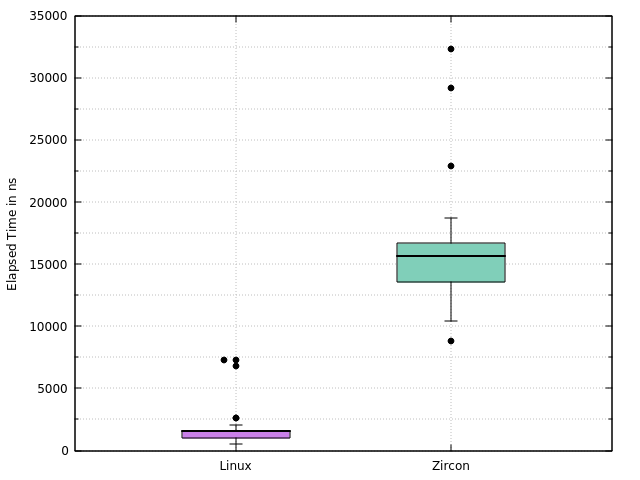
\includegraphics[width=\linewidth]{perfcomp-gnuplot}
    \caption{Performance Comparison between Linux and Zircon}\label{pic:perftest}
\end{figure}

The resulting values for Linux and Zircon are pictured as a \textit{box-plot} in figure~\ref{pic:perftest}.
This diagram type allows a comparable statistical representation of the elapsed time in nanoseconds.
Each colored box has the size of the interquartile range (IQR) for the given values.
It contains the average 50\% of the datapoints limited by the upper and lower quartile.
The bigger line within a box represents the median for the given range.
The lines starting at the box are named \textit{whiskers} and picture the range from the last values within the $1.5 * IQR$ below and above the box.
Values within this range are also named as milde outlier values in contrast to the ones outside, pictured as dots. 

Figure~\ref{pic:perftest} shows a significat difference in the time needed to toggle a \ac{gpio}.
The overall span of measured results but especially the box height in Linux is much smaller than in Zircon.
All in all ranged the Linux values between 520 and 7291 ns with a median on 1562 ns.
For Zircon, the overall span starts higher, on 8854 ns which is clearly above than the outlier values on Linux.
At the same time takes the box height as well as the span a wider range with a median on 15625 ns and extreme outliers on up to 32291 ns.
Considering the median values is Zircons \mintinline{c}{gpio_write()} approximately 10 times slower than Linux' \mintinline{c}{gpio_set_value()}.
However, the way this difference in performance is exactly influenced by various factors such as the used development board revisions, the scheduling strategies and the additional context changes in the microkernel approch, which is assumed to be a major factor, can not be deducated from the measurement.
Based on the results of this measurement, it can of course be assumed that the overall performance of both systems behaves similarly in comparison.
But for reliable statements are more in-depth and comprehensive tests neccessary.

